\documentclass[twocolumn]{article}

\usepackage{lipsum} 
\usepackage{hyperref}
\usepackage{placeins}
%\hypersetup{colorlinks,urlcolor=blue}
\hypersetup{colorlinks,urlcolor=black}

\usepackage{graphicx}

\title{Modelling Covid spread and travel using a problem specific formalism implemented in PDEVS}
\author{Griffin Barrett}

\graphicspath{ {./images/} }

\begin{document}

\twocolumn[
\begin{@twocolumnfalse}
	\maketitle
	\begin{abstract}
		\begin{center}
		Over the Fall 2020 term, I worked on generalizing a PDEVS Covid model that I had made the previous summer. This report talks about the direction that effort took and the new tech that came out if it.
		\end{center}
	\end{abstract}
\end{@twocolumnfalse}
]
\clearpage
\section{Introduction}

Over the summer of 2020, many Covid spread models were developed by the lab using PDEVS. These models all fell into one of two camps. They ether had very sophisticated modelling for one territory, but did not model travel, or they had the most basic modelling for each territory, but had sophisticated travel and migration models. This project grew out of trying to take one from the first camp, and grow it into one that can do both, and has become a problem-specific formalism of sorts.

\section{Multi-Paradigm Modelling}

\FloatBarrier

Multi-paradigm modelling[1] is a technique where instead of writing an entire simulator in one language with one tool under one formalism, you write different parts of that simulator in the way that is the most useful locally, and you use some more general set of tools to link them together.

You can see something like this whenever you write a program in more than one language, or in one language making calls into a library written in another language. In the case of programming, the common ground that is used to connect these parts is usually the operating system and machine code. In the more formal world of modelling, the common ground is some modelling formalism that can be used to fully describe all of the disparate parts of the simulator in question.

\begin{figure}[!ht]
	\begin{center}
		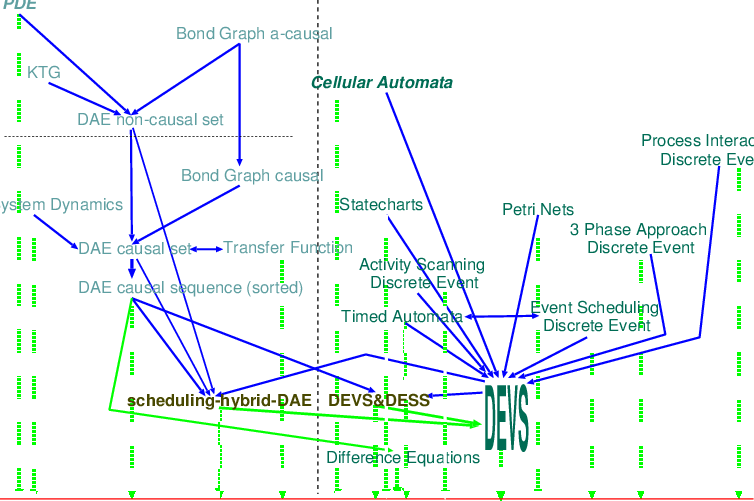
\includegraphics[width=18em]{Formalism-Transformation-Graph-FTG.png}
		\caption{Formalism Transformation Graph (FTG)[1]}
		\label{fig:ftg}
	\end{center}
\end{figure}

% How many papers/reports/presentations do you think start with 'Figure 1, Formalism Transformation Graph (FTG)'?

Figure \ref{fig:ftg} is a directed graph of which simulation formalisms have been proven to be able to describe which others. When linking any set of systems together, you need to find some common super-formalism to describe everything in. For any combination, that includes only formalisms that are either naturally discreet, or can reasonably be discretised, the DEVS family of formalisms can be used as this super-formalism.

\FloatBarrier

\subsection{DEVS}

DEVS represents everything within the simulation frame as ether an atomic model, or as a collection of connected models called a coupled model, and represents everything that can happen within the simulation frame as a transition. Transitions that a model applies to itself internally called internal transitions, and transitions that one model apply to another model, or that one model apply to itself using the external communication mechanism, are called external transitions.

Each atomic model describes it's state, the set of types of messages that it can receive, the set of types of messages that it can send, and the five functions that are required of it. These functions are: the internal transition function, the external transition function, the confluent function for cases where both the internal and external are fired at the same time, the output function, and the time advance function. 

Each coupled model describes how the models that it contains are interconnected, what types of inputs and outputs the coupled model handles, and what order to run the functions of the sub models.

All of this is sufficiently powerful and general to implement just about anything that we could want to represent, but this comes at the cost of the pieces being small and fiddly. This positions it in roughly the same place as machine code is relative to general computer programs. You \textit{can} to just about anything with it, but if there are tools to smooth out the rough edges, they can be used to great effect in speeding up the development process.

\section{My Formalism}

My formalism, that is yet unnamed, is built on top of PDEVS, which itself is an extension of DEVS that handles simultaneous events more naturally. It can be thought of in the same way any of the many formalisms in figure \ref{fig:ftg} that are directly described by DEVS. It is more narrow than DEVS, but with that it also has fewer and more simple parts that the modeller needs to work with by hand.

\subsection{Design}

If we consider only modelling the movement of people between territories, what do we need? We need something to represent the territory, some way to represent people that are moving, and some way to work out how many people should move. Lets start with the simplest possible implementation of that, a number for people in an area, a number for people moving, and a proportion between 0 and 1 of the population in an area that are going to leave in a time step.

\begin{verbatim}
<
  id::ID
  pop::REAL
  travel_rates::MAP<::ID, ::REAL>
>::DIST

local_advance(dist::DIST):
| output::MAP<::ID, ::DELTA> = {}
| 
| for id, travel in dist.travel_rates:
| | output[id] = dist.pop*travel
| 
| for _, left in output:
| | dist.pop = dist.pop - left
|
| return output

local_apply(
|   dist::DIST, 
|   deltas::SET<::DELTA>
|   ):
| for delta in deltas:
| | dist.pop = 
| |   dist.add(dist.pop, delta)

global_advance(
|   dists::MAP<::ID, ::DIST>,
|   ):
| messages::MAP<::ID, ::SET<::DELTA>> = {}
| 
| for _, dist in dists:
| | for id, delta in 
| | |   local_advance(dist):
| | | messages[id].add(delta)
| 
| for id, deltas in messages:
| | local_apply(dists[id], deltas)

\end{verbatim}

Ok, this works, but the extra loop at the end of $local_advance$ to remove the people that left is a bit inelegant. What if, instead of doing that, when we send a group of people away, we also send the negation of that group back to where they came? That way, the subtraction happens in $local_collect$ instead.

Now $local_advance$ looks like this:

\begin{verbatim}

local_advance(dist::DIST):
| output::MAP<::ID, ::DELTA> = {}
| delta_pop = 0
| 
| for id, travel in dist.travel_rates:
| | delta_travel = dist.pop*travel
| | output[id] = delta_travel
| | delta_pop = delta_pop - delta_travel 
|
| output[dist.id] = delta_pop
|
| return output

\end{verbatim}

That looks better. Now, how do we model the population in a territory changing over time? 
Lets start with the most simple version of this that we can think of, a proportion of people die every time step.
What would it look like if, instead of starting $delta_pop$ at 0, we started it at a value that represents the amount that the population changes on it's own?
That way, when it gets re-applied in $local_collect$, the change happens simultaneously with the people leaving.

\begin{verbatim}

<
  id::ID
  pop::REAL
  death_rate::REAL
  travel_rates::MAP<::ID, ::REAL>
>::DIST

local_advance(dist::DIST):
| output::MAP<::ID, ::DELTA> = {}
| delta_pop = -dist.pop*dist.death_rate
| 
| for id, travel in dist.travel_rates:
| | delta_travel = dist.pop*travel
| | output[id] = delta_travel
| | delta_pop = delta_pop - delta_travel 
|
| output[dist.id] = delta_pop
|
| return output
	
\end{verbatim}

This is starting to come together, now lets generalize. First thing to go is the assumption that the time step is 1. Lets add in a value for delta time.

\begin{verbatim}

local_advance(dist::DIST, dt::REAL):
| output::MAP<::ID, ::DELTA> = {}
| delta_pop = -dist.pop*dist.death_rate*dt
| 
| for id, travel in dist.travel_rates:
| | delta_travel = dist.pop*travel*dt
| | output[id] = delta_travel
| | delta_pop = delta_pop - delta_travel 
|
| output[dist.id] = delta_pop
|
| return output
	
\end{verbatim}

Now we have all the pieces in place. The next and last step is to go through and pull out all of the decisions. Instead of using real numbers for everything, we will allow any value of any consistent set of types. When we do that, we also need to allow the multiplication, addition, and subtraction in out system to be replaced with other functions that take and give the correct types. These changes take us right up to the final version described in full in the next sections.

\subsection{Informal}

This technique encapsulates the local computation in a territory into a thing called a district. 
A district can represent anything from a house, to a block, to a city or country.
Each district has a way of representing the population of people within it, and any other parameters that change over short spans of time.
Each district also has a way of representing a change in that population. This is something that districts must agree on in order to be connected to one another.
Each district also has it's own computational model for computing the change in that population over time. 
That local computation can use a set of constant parameters to hold information that does not change, stored locally within the district.
Districts also contain the local computation that represents how many people leave the territory over time. This likewise can leverage a set of parameters, this time local to the district and the name of the destination.

It is normal to have many districts in a global model that only vary in the parameters that they store and the connections that they have, though this is not a requirement. The only thing that requires global agreement is the way that districts are identified, and the way that changes in population are represented.

A later development in this project was to add the ability to poke the otherwise constant parameters of a district. This was done to make modelling changes of policy at fixed points in time easier.

\subsection{Formal}

This is the formal description of all of the parts of this formalism that are prescribed. The specifics of all of the listed types are left up to the implementer and modeller other than the fact that the required operations much be well defined over the range of values that come up during simulation.

\begin{verbatim}
<
  ID::TYPE, 
  POP::TYPE, 
  DELTA::TYPE, 
  PARAMS::TYPE, 
  TRAVEL::TYPE, 
  TIME::TYPE,
  
  id::ID, 
  pop::POP, 
  params::PARAMS, 
  travel_rates::MAP<::ID, ::TRAVEL>, 
  
  delta(::PARAMS, ::POP, ::TIME)::DELTA, 
  travel(::TRAVEL, ::POP, ::TIME)::DELTA, 
  add(::POP, ::DELTA)::POP, 
  subtract(::DELTA, ::DELTA)::DELTA
>::DIST

local_advance(dist::DIST, dt::TIME):
| output::MAP<::ID, ::DELTA> = {}
| delta_pop = 
| | dist.delta(dist.params, dist.pop, dt)
| 
| for id, travel in dist.travel_rates:
| | delta_travel = 
| |   dist.travel(travel, dist.pop, dt)
| | 
| | output[id] = delta_travel
| | delta_pop = 
| |   dist.subtract(
| |       delta_pop, 
| |       delta_travel
| |       )
| 
| output[dist.id] = delta_pop
| return output
  
local_apply(
|   dist::DIST, 
|   deltas::SET<::DELTA>
|   ):
| for delta in deltas:
| | dist.pop = 
| |   dist.add(dist.pop, delta)

global_advance(
|   dists::MAP<::ID, ::DIST>, 
|   dt::TIME
|   ):
| messages::MAP<::ID, ::SET<::DELTA>> = {}
| 
| for _, dist in dists:
| | for id, delta in 
| | |   local_advance(dist, dt):
| | | messages[id].add(delta)
| 
| for id, deltas in messages:
| | local_apply(dists[id], deltas)
 
\end{verbatim}

\subsection{PDEVS implementation}

This is formal definition for the sample implementation of my formalism. This may not be the best way to implement it in general, and it may not even be the best way to implement it in PDEVS, but that is for the software engineers to argue about. For now, it works and at this stage in it's development that is good enough.

\begin{verbatim}

Givin some district D, 
the PDEVS atomic model to represent it
is the following

<
  S:{
    id::D.ID,
    pop::D.POP,
    params::D.PARAMS,
    travel_rates::MAP<::D.ID, ::D.TRAVEL>,
    dt::TIME,
    time_till_report::TIME
  },

  X:{
    people_in ::PAIR<::D.ID, ::D.POP>,
    new_params ::PAIR<::D.ID, ::D.PARAMS>,
    new_travel_rate::TUPLE<
        source::D.ID, 
        destination::D.ID, 
        ::D.PARAMS
        >
  },

  Y:{
    report::D.POP,
    people_out::PAIR<::D.ID, ::D.DELTA>
  },

  int:(){
  |   state.time_till_report = state.dt
  },

  ext:(t::TIME, mbs::INPUTS){
  |   state.time_till_report -= t
  |   
  | for src, dest, travel
  | |   in mbs.new_travel_rate:
  | | if state.id == src:
  | | | state.travel_rates[dest] = travel
  |     
  | for id, params in mbs.new_params:
  | | if state.id == id:
  | | | state.params = params
  | 
  | for id, delta in state.people_in:
  | | if state.id = id:
  | | | state.pop = 
  | | |     D.add(state.pop, delta)
  },

  confluent:(t::TIME, mbs::INPUTS){
  | int()
  | ext(0, mbs)
  },
 
  output:(){
  | output = make_output_bags()
  |	
  |	output.report.add(state.pop)
  |	
  | delta = D.delta(
  |     state.params, 
  |     state.pop, 
  |     state.dt
  |     )
  | for dest, travel in state.travel_rates:
  | | tr = D.travel(travel, state.pop, dt)
  | | output.people_out.add(dest, tr)
  | | delta = D.subtract(delta, tr)
  | 
  | output.people_out.add(state.id, delta)
  | 
  | return output
  },

  ta:{
  | return state.time_till_report
  }
>

\end{verbatim}

Each district model \textbf{must} have it's $people\_ou$t connected to it's own $people\_in$. 
For each element in a given district's $travel\_rates$, it \textbf{should} have some model that listens to that element's id connected to that district's $people\_out$. 
There \textbf{should not} be duplicated $id$s, and districts with duplicate $id$s \textbf{must not} be connected.

\section{Results}
\FloatBarrier

To test out that this formalism can work, I re-implemented the model from the summer in it, and compared it back to the original paper that all of this model's computational method is based on. As you can see in figure \ref{fig:overlay}, the output perfectly lines up with the diagram from the first paper, to within the resolution of the diagrams provided by that paper.

\begin{figure}[!ht]
	\begin{center}
		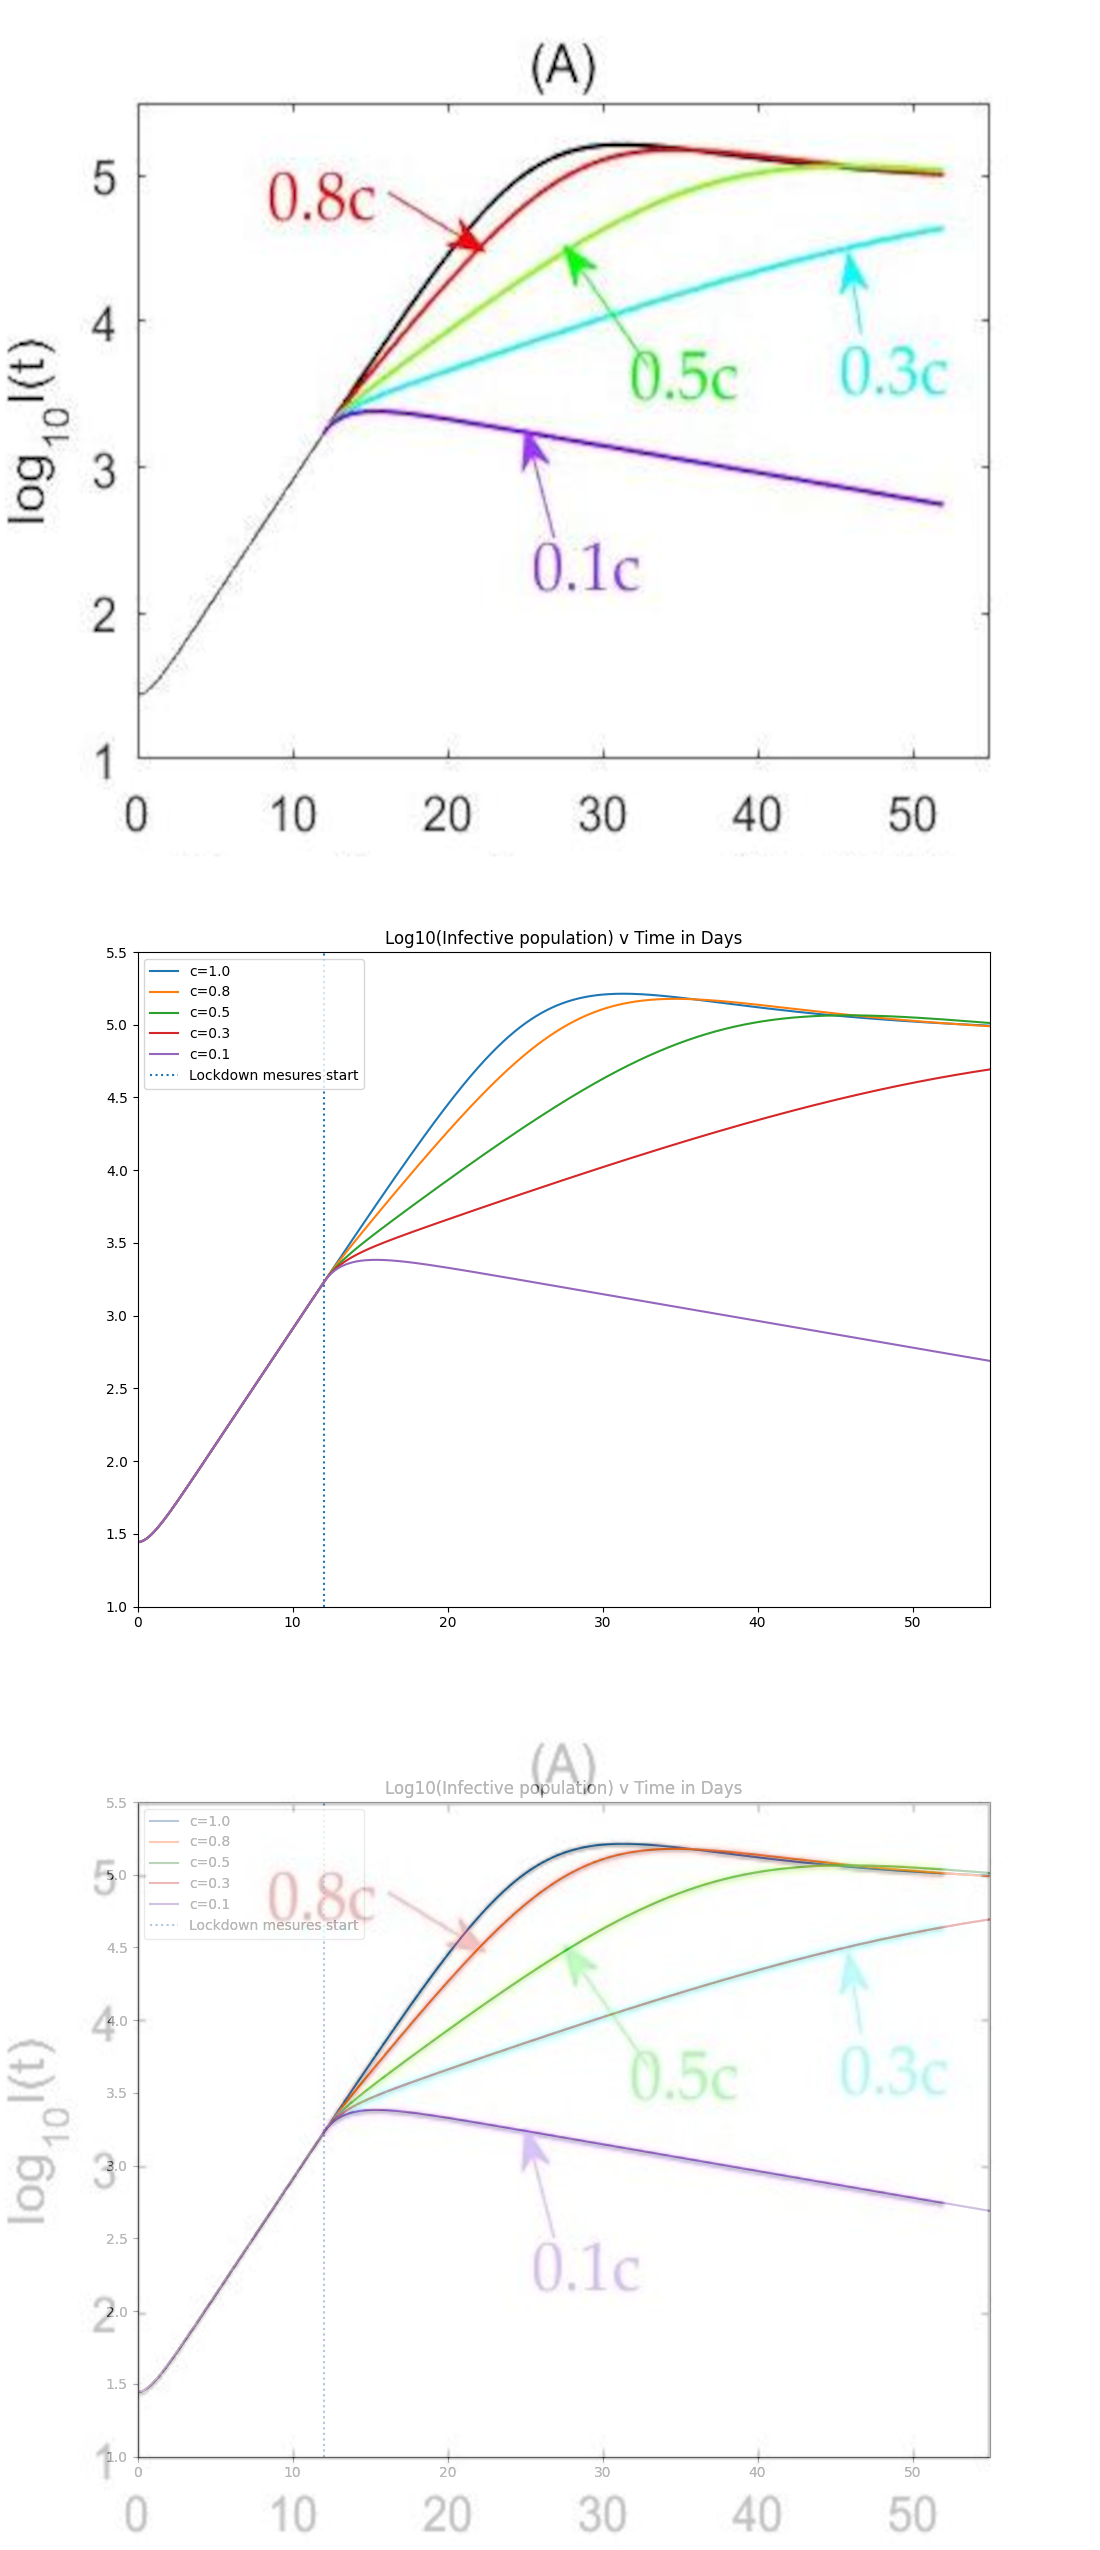
\includegraphics[width=18em]{figure_a_overlay.png}
		\caption{Figure A from original paper[2] (Top), Output from reimplementation (Middle), An overlay to scale of both figures (Bottom)}
		\label{fig:overlay}
	\end{center}
\end{figure}


\FloatBarrier
\section{Improvements and Future Work}

The current implementation of these tools require that the structure and initial values of the model be hardcoded. This does not represent a fundamental limitation on these techniques, and is an area of future technical development, with the designing of a file format to describe these models and the appropriate parsers and constructors to use this information to lay out a model at run time. 

Another area of development is the formatting of the output. Unlike generalized PDEVS, under the constraints imposed by this formalism, it may be possible to create a generalized and meaningful output parser. The existing $plotter.py$ family of scripts that come bundled with the implementation may be the start of this, or perhaps it will take some other form.

This formalism is compostable, but it is not modular at any scale above a single district. There may be value in also defining a kind of meta district that contains some number of others. It remains to be seen if this will actually be useful at runtime, as opposed to simply flattening the model at construction time, but it should be implemented and tested before it is discarded.

\section{Code}

The code for the first implementation of all of this can be found here: \url{https://github.com/xlirate/Cadmin-Cell-DEVS-SAMC}.
It is built on top of the Cadmium simulation library, which can be found here: \url{https://github.com/SimulationEverywhere/cadmium}.

See \url{http://www.sce.carleton.ca/courses/sysc-5104/lib/exe/fetch.php?media=cadmiumusermanual.pdf} for instructions on how to set it up.

\section{Bibliography}

\begin{enumerate}

\item Lara, Juan \& Vangheluwe, Hans. (2002). Computer Aided Multi-paradigm Modelling to Process Petri-Nets and Statecharts. 239-253. 10.1007/3-540-45832-8\_19. \url{http://dx.doi.org/10.1007/3-540-45832-8_19}

\item Tang, B., Wang, X., Li, Q., Bragazzi, N. L., Tang, S., Xiao, Y., \& Wu, J. (2020).
Estimation of the Transmission Risk of the 2019-nCoV and Its Implication for
Public Health Interventions. Journal of clinical medicine, 9(2), 462.
\url{https://doi.org/10.3390/jcm9020462}

\end{enumerate}

\end{document}








